\documentclass[10pt]{beamer}\usepackage[]{graphicx}\usepackage[]{color}
%% maxwidth is the original width if it is less than linewidth
%% otherwise use linewidth (to make sure the graphics do not exceed the margin)
\makeatletter
\def\maxwidth{ %
  \ifdim\Gin@nat@width>\linewidth
    \linewidth
  \else
    \Gin@nat@width
  \fi
}
\makeatother

\definecolor{fgcolor}{rgb}{0.345, 0.345, 0.345}
\newcommand{\hlnum}[1]{\textcolor[rgb]{0.686,0.059,0.569}{#1}}%
\newcommand{\hlstr}[1]{\textcolor[rgb]{0.192,0.494,0.8}{#1}}%
\newcommand{\hlcom}[1]{\textcolor[rgb]{0.678,0.584,0.686}{\textit{#1}}}%
\newcommand{\hlopt}[1]{\textcolor[rgb]{0,0,0}{#1}}%
\newcommand{\hlstd}[1]{\textcolor[rgb]{0.345,0.345,0.345}{#1}}%
\newcommand{\hlkwa}[1]{\textcolor[rgb]{0.161,0.373,0.58}{\textbf{#1}}}%
\newcommand{\hlkwb}[1]{\textcolor[rgb]{0.69,0.353,0.396}{#1}}%
\newcommand{\hlkwc}[1]{\textcolor[rgb]{0.333,0.667,0.333}{#1}}%
\newcommand{\hlkwd}[1]{\textcolor[rgb]{0.737,0.353,0.396}{\textbf{#1}}}%
\let\hlipl\hlkwb

\usepackage{framed}
\makeatletter
\newenvironment{kframe}{%
 \def\at@end@of@kframe{}%
 \ifinner\ifhmode%
  \def\at@end@of@kframe{\end{minipage}}%
  \begin{minipage}{\columnwidth}%
 \fi\fi%
 \def\FrameCommand##1{\hskip\@totalleftmargin \hskip-\fboxsep
 \colorbox{shadecolor}{##1}\hskip-\fboxsep
     % There is no \\@totalrightmargin, so:
     \hskip-\linewidth \hskip-\@totalleftmargin \hskip\columnwidth}%
 \MakeFramed {\advance\hsize-\width
   \@totalleftmargin\z@ \linewidth\hsize
   \@setminipage}}%
 {\par\unskip\endMakeFramed%
 \at@end@of@kframe}
\makeatother

\definecolor{shadecolor}{rgb}{.97, .97, .97}
\definecolor{messagecolor}{rgb}{0, 0, 0}
\definecolor{warningcolor}{rgb}{1, 0, 1}
\definecolor{errorcolor}{rgb}{1, 0, 0}
\newenvironment{knitrout}{}{} % an empty environment to be redefined in TeX

\usepackage{alltt}%
\usetheme{Boadilla}
\usecolortheme{seahorse}

\usepackage[utf8]{inputenc}%


\usepackage[normalem]{ulem}%strikeout
 

% graphics
%% Figures %%%%%%%%%%%%%%%%%%%%%%%%%%%%%%%%%%%%%%%%%%%%%%%%%%
\usepackage{graphicx}
\usepackage{xcolor}%for color mixing

\usepackage{amsmath}%
\usepackage{amsfonts}%
\usepackage{amssymb}%
\usepackage{graphicx}

\usepackage{tikz}
\usetikzlibrary{calc}

%%%%%%%%%%%%%%%%%%%%%%%%%%%%%%%%%%%%%%%%%%%%%%
%%%%%%%%%%%%%%%%% Doc info %%%%%%%%%%%%%%%%%%%
\title[\textbf{Linear models 3:}]{Multiple regressions and interactions}
\date{\today}

%%%%%%%%%%%%%%%%%%%%%%%%%%%%%%%%%%%%
\IfFileExists{upquote.sty}{\usepackage{upquote}}{}
\begin{document}




\begin{frame}
\maketitle
\end{frame}
%%%%%%%%%%%

\AtBeginSection[]
{
  \begin{frame}<beamer>
    \frametitle{}
    \tableofcontents[currentsection,hideothersubsections,subsectionstyle=hide]% down vote\tableofcontents[currentsection,currentsubsection,hideothersubsections,sectionstyle=show/hide,subsectionstyle=show/shaded/hide]
  \end{frame}
}



%%%%%%%%%%%%%%%%%%%%%%%%%%%%%%%%%%%%%%%%%%%%%%%%%%%%%%%%%%%%%%%%%%%
%%%%%%%%%%%%%%%%%%%%%%%%%%%%%%%%%%%%%%%%%%%%%%%%%%%%%%%%%%%%%%%%%%%
\section{Linear model, reminder}

\begin{frame}[fragile]{A simple linear model}
  \textbf{{\color{purple}{Response}} = {\color{blue}{Intercept}} + {\color{red}{Slope}} $\times$ {\color{orange}{Predictor}} + {\color{gray}{Error}}} \\

\begin{knitrout}\small
\definecolor{shadecolor}{rgb}{0.843, 0.867, 0.922}\color{fgcolor}
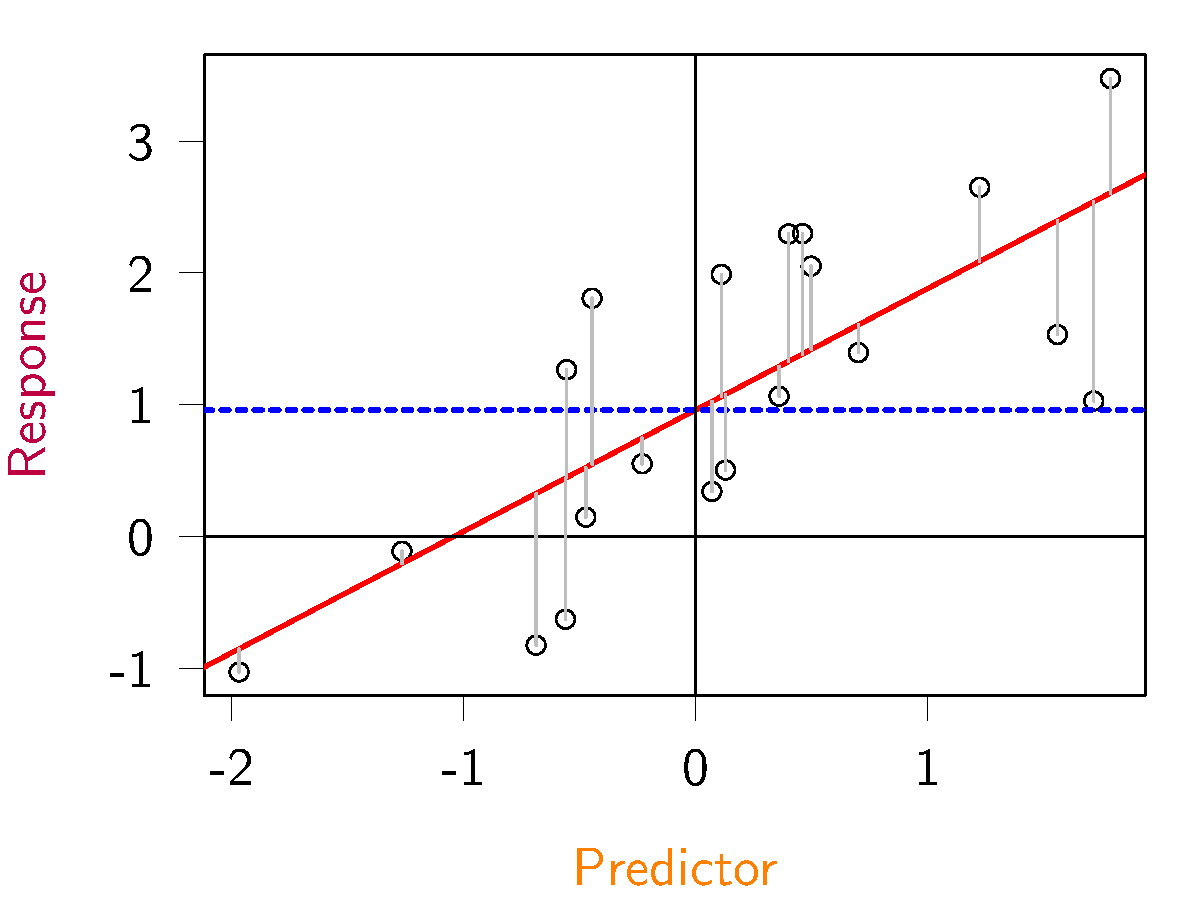
\includegraphics[width=0.8\textwidth,height=0.6\textwidth]{figure/lmprinc-1} 

\end{knitrout}
\end{frame}
%%%%%%%%%%%

\begin{frame}[fragile]{A multiple linear model}
  \textbf{{\color{purple}{Response}} = {\color{blue}{Intercept}} + {\color{red}{Slope1}} $\times$ {\color{orange}{Predictor1}} + {\color{red}{Slope2}} $\times$ {\color{orange}{Predictor2}}  + {\color{gray}{Error}}} \\
  \vspace{1cm}
\textbf{In R:}
\begin{knitrout}\small
\definecolor{shadecolor}{rgb}{0.843, 0.867, 0.922}\color{fgcolor}\begin{kframe}
\begin{alltt}
  \hlkwd{lm}\hlstd{(response} \hlopt{~} \hlnum{1} \hlopt{+} \hlstd{predictor1} \hlopt{+} \hlstd{predictor2,} \hlkwc{data}\hlstd{=data)}
\end{alltt}
\end{kframe}
\end{knitrout}


\end{frame}
%%%%%%%%%%%

%%%%%%%%%%%%%%%%%%%%%%%%%%%%%%%%%%%%%%%%%%%%%%%%%%%%%%%%%%%%%%%%%%%%%%%%%%%%%%%%%%%%%%%%%%%%%%%%%%%%
\section{Multiple regression}

\begin{frame}[fragile]{Sequential regression}


  
We want to explain a response by three predictors
\only<2>{
\begin{knitrout}\small
\definecolor{shadecolor}{rgb}{0.843, 0.867, 0.922}\color{fgcolor}
\includegraphics[width=0.8\textwidth,height=0.6\textwidth]{figure/lmprinc1-1} 

\end{knitrout}
}
\only<3>{
\begin{knitrout}\small
\definecolor{shadecolor}{rgb}{0.843, 0.867, 0.922}\color{fgcolor}
\includegraphics[width=0.8\textwidth,height=0.6\textwidth]{figure/lmprinc2-1} 

\end{knitrout}
}
\only<4>{
\begin{knitrout}\small
\definecolor{shadecolor}{rgb}{0.843, 0.867, 0.922}\color{fgcolor}
\includegraphics[width=0.8\textwidth,height=0.6\textwidth]{figure/lmprinc3-1} 

\end{knitrout}
}

\end{frame}
%%%%%%%%%%%

\begin{frame}[fragile]{Sequential regression}

\begin{knitrout}\small
\definecolor{shadecolor}{rgb}{0.843, 0.867, 0.922}\color{fgcolor}\begin{kframe}
\begin{alltt}
  \hlstd{m1} \hlkwb{<-} \hlkwd{lm}\hlstd{(y} \hlopt{~} \hlstd{x1)}
  \hlstd{m2} \hlkwb{<-} \hlkwd{lm}\hlstd{(m1}\hlopt{$}\hlstd{residuals} \hlopt{~} \hlstd{x2)}
  \hlstd{m3} \hlkwb{<-} \hlkwd{lm}\hlstd{(m2}\hlopt{$}\hlstd{residuals} \hlopt{~} \hlstd{x3)}
\end{alltt}
\end{kframe}
\end{knitrout}
\end{frame}
%%%%%%%%%%%

\begin{frame}[fragile]{Sequential regression}

But, 
\begin{knitrout}\small
\definecolor{shadecolor}{rgb}{0.843, 0.867, 0.922}\color{fgcolor}\begin{kframe}
\begin{alltt}
  \hlstd{m1} \hlkwb{<-} \hlkwd{lm}\hlstd{(y} \hlopt{~} \hlstd{x1)}
  \hlstd{m2} \hlkwb{<-} \hlkwd{lm}\hlstd{(m1}\hlopt{$}\hlstd{residuals} \hlopt{~} \hlstd{x2)}
  \hlstd{m3} \hlkwb{<-} \hlkwd{lm}\hlstd{(m2}\hlopt{$}\hlstd{residuals} \hlopt{~} \hlstd{x3)}

  \hlkwd{coefficients}\hlstd{(m1);} \hlkwd{coefficients}\hlstd{(m2);} \hlkwd{coefficients}\hlstd{(m3)}
\end{alltt}
\begin{verbatim}
(Intercept)          x1 
  0.4585067   0.4715738 
(Intercept)          x2 
-0.02542972  0.75420781 
 (Intercept)           x3 
-0.009178959  0.257305942 
\end{verbatim}
\end{kframe}
\end{knitrout}
is different from
\begin{knitrout}\small
\definecolor{shadecolor}{rgb}{0.843, 0.867, 0.922}\color{fgcolor}\begin{kframe}
\begin{alltt}
    \hlstd{m1} \hlkwb{<-} \hlkwd{lm}\hlstd{(y} \hlopt{~} \hlstd{x3)}
    \hlstd{m2} \hlkwb{<-} \hlkwd{lm}\hlstd{(m1}\hlopt{$}\hlstd{residuals} \hlopt{~} \hlstd{x2)}
    \hlstd{m3} \hlkwb{<-} \hlkwd{lm}\hlstd{(m2}\hlopt{$}\hlstd{residuals} \hlopt{~} \hlstd{x1)}

    \hlkwd{coefficients}\hlstd{(m1);} \hlkwd{coefficients}\hlstd{(m2);} \hlkwd{coefficients}\hlstd{(m3)}
\end{alltt}
\begin{verbatim}
(Intercept)          x3 
  0.5289919  -0.1036939 
(Intercept)          x2 
-0.03288572  0.97534187 
(Intercept)          x1 
 0.01443407 -0.10191840 
\end{verbatim}
\end{kframe}
\end{knitrout}
\end{frame}
%%%%%%%%%%%
\begin{frame}[fragile]{Sequential regression}

  Also what happens with classical ANOVA (aov in R)
  
\begin{knitrout}\small
\definecolor{shadecolor}{rgb}{0.843, 0.867, 0.922}\color{fgcolor}\begin{kframe}
\begin{alltt}
  \hlkwd{summary}\hlstd{(}\hlkwd{aov}\hlstd{(y} \hlopt{~} \hlstd{x1} \hlopt{+} \hlstd{x2} \hlopt{+} \hlstd{x3))}
\end{alltt}
\begin{verbatim}
            Df Sum Sq Mean Sq F value   Pr(>F)    
x1           1  3.997   3.997  394.05 1.07e-12 ***
x2           1 13.998  13.998 1379.87  < 2e-16 ***
x3           1  0.120   0.120   11.82  0.00338 ** 
Residuals   16  0.162   0.010                     
---
Signif. codes:  0 '***' 0.001 '**' 0.01 '*' 0.05 '.' 0.1 ' ' 1
\end{verbatim}
\begin{alltt}
  \hlkwd{summary}\hlstd{(}\hlkwd{aov}\hlstd{(y} \hlopt{~} \hlstd{x2} \hlopt{+} \hlstd{x3} \hlopt{+} \hlstd{x1))}
\end{alltt}
\begin{verbatim}
            Df Sum Sq Mean Sq  F value  Pr(>F)    
x2           1 17.931  17.931 1767.562 < 2e-16 ***
x3           1  0.183   0.183   18.003 0.00062 ***
x1           1  0.002   0.002    0.176 0.68076    
Residuals   16  0.162   0.010                     
---
Signif. codes:  0 '***' 0.001 '**' 0.01 '*' 0.05 '.' 0.1 ' ' 1
\end{verbatim}
\end{kframe}
\end{knitrout}
\end{frame}
%%%%%%%%%%%

\begin{frame}[fragile]{Multiple regression}
In contrast lm() optimizes relationships simultaneously\\
Order does \textbf{not} matter:
\begin{knitrout}\small
\definecolor{shadecolor}{rgb}{0.843, 0.867, 0.922}\color{fgcolor}\begin{kframe}
\begin{alltt}
  \hlkwd{coefficients}\hlstd{(}\hlkwd{lm}\hlstd{(y} \hlopt{~} \hlstd{x1} \hlopt{+} \hlstd{x2} \hlopt{+} \hlstd{x3))}
\end{alltt}
\begin{verbatim}
(Intercept)          x1          x2          x3 
 0.48948612 -0.01357404  1.03015700  0.08395938 
\end{verbatim}
\begin{alltt}
  \hlkwd{coefficients}\hlstd{(}\hlkwd{lm}\hlstd{(y} \hlopt{~} \hlstd{x2} \hlopt{+} \hlstd{x3} \hlopt{+} \hlstd{x1))}
\end{alltt}
\begin{verbatim}
(Intercept)          x2          x3          x1 
 0.48948612  1.03015700  0.08395938 -0.01357404 
\end{verbatim}
\end{kframe}
\end{knitrout}

\end{frame}
%%%%%%%%%%%

\begin{frame}[fragile]{Multiple regression}
\textbf{BUT} estimates may change with extra covariates
\begin{knitrout}\small
\definecolor{shadecolor}{rgb}{0.843, 0.867, 0.922}\color{fgcolor}\begin{kframe}
\begin{alltt}
    \hlkwd{coefficients}\hlstd{(}\hlkwd{lm}\hlstd{(y} \hlopt{~} \hlstd{x1} \hlopt{+} \hlstd{x2 ))}
\end{alltt}
\begin{verbatim}
(Intercept)          x1          x2 
 0.50022999 -0.07029467  1.03858671 
\end{verbatim}
\begin{alltt}
    \hlkwd{coefficients}\hlstd{(}\hlkwd{lm}\hlstd{(y} \hlopt{~} \hlstd{x1} \hlopt{+} \hlstd{x2} \hlopt{+} \hlstd{x3))}
\end{alltt}
\begin{verbatim}
(Intercept)          x1          x2          x3 
 0.48948612 -0.01357404  1.03015700  0.08395938 
\end{verbatim}
\end{kframe}
\end{knitrout}
\pause
\begin{block}{??}
  \begin{itemize}
    \item That is a good thing
    \item Estimates are independent effects, conditional on the other parameters
  \end{itemize}
\end{block}
\end{frame}
%%%%%%%%%%%

\begin{frame}[fragile]{Conditional estimation}

\begin{exampleblock}{Exercise}
  \begin{enumerate}
    \item load jumpingdistance.csv
    \item Use plots and lm() to test whether mass increases jumping distance
  \end{enumerate}
\end{exampleblock}



\begin{knitrout}\small
\definecolor{shadecolor}{rgb}{0.843, 0.867, 0.922}\color{fgcolor}\begin{kframe}
\begin{alltt}
  \hlstd{jumping} \hlkwb{<-} \hlkwd{read.csv}\hlstd{(}\hlkwc{file} \hlstd{=} \hlstr{"jumpingdistance.csv"}\hlstd{)}
\end{alltt}
\end{kframe}
\end{knitrout}
  
  
\end{frame}
%%%%%%%%%%%

\begin{frame}{Conditional estimation}
  \begin{center}
  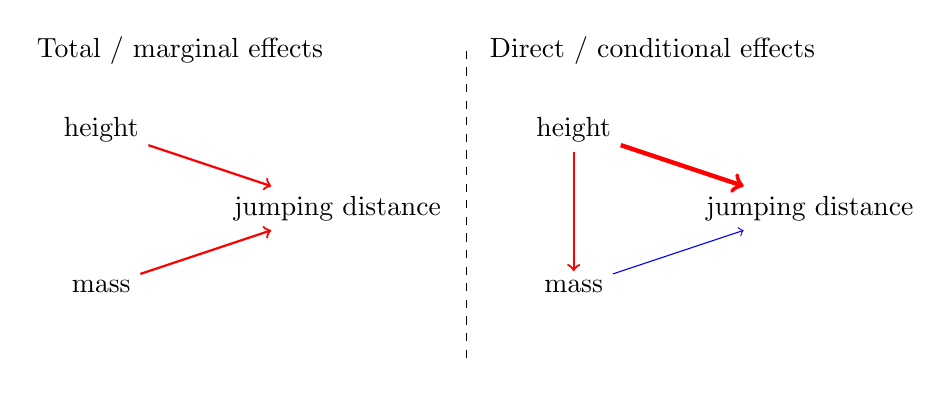
\begin{tikzpicture}
  \node (cor) at (-8, 2) {Total / marginal effects};
    \node (jump1) at (-6,0) {jumping distance};
    \node (height1) at (-9, 1) {height};
    \node (mass1) at (-9, -1) {mass};
    \draw[->, thick, color=red] (height1) -- (jump1);
    \draw[->, thick, color=red] (mass1) -- (jump1);

  \draw[dashed] ($(jump1.east)+(0.2,2)$)-- ($(jump1.east)+(0.2,-2)$);
  
  \pause
  
    \node (caus) at (-2, 2) {Direct / conditional effects};
    \node (jump) at (0,0) {jumping distance};
    \node (height) at (-3, 1) {height};
    \node (mass) at (-3, -1) {mass};
    \draw[->, ultra thick, color=red] (height) -- (jump);
    \draw[->, color=blue] (mass) -- (jump);
    \draw[->, color=red, thick] (height)--(mass);
  \end{tikzpicture}
  \end{center}
  
  \pause
  \begin{itemize}
    \item Marginal effects $\approx$ raw correlations, sum of direct and indirect effects
    \item Multiple regression estimates direct effects may reveal causal relationships
  \end{itemize}
\end{frame}
%%%%%%%%%%%

\begin{frame}{Conditional estimation}
  \begin{exampleblock}{Exercise}
  \end{exampleblock}
\end{frame}
%%%%%%%%%%%

\begin{frame}[fragile]{Conditional estimation final warning: more is not always better}

  
  \textbf{Are more innovative papers less rigorous?}
  \begin{center}
  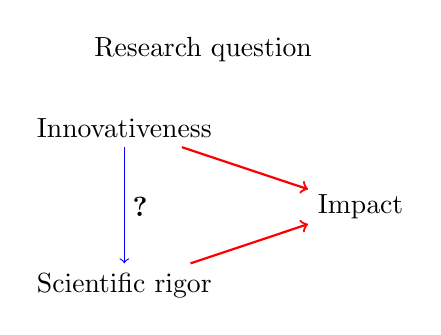
\begin{tikzpicture}
    \node (cor) at (-8, 2) {Research question};
    \node (rig) at (-9,-1) {Scientific rigor};
    \node (innov) at (-9, 1) {Innovativeness};
    \draw[->, color=blue] (innov)--(rig);
    \node (qm) at (-8.8,0) {\textbf{?}};
    
    \pause
    \node (impact) at (-6, 0) {Impact};
    \draw[->, color=red, thick] (rig)--(impact);
    \draw[->, color=red, thick] (innov)--(impact);
    
  \end{tikzpicture}
  \end{center}
  
  \textit{Should you correct for publication impact?}
  
\end{frame}
%%%%%%%%%%%

\begin{frame}[fragile]{Conditional estimation final warning: more is not always better}
    \textit{Should you include publication impact?}
\begin{knitrout}\small
\definecolor{shadecolor}{rgb}{0.843, 0.867, 0.922}\color{fgcolor}\begin{kframe}
\begin{alltt}
    \hlkwd{summary}\hlstd{(}\hlkwd{lm}\hlstd{(rigor} \hlopt{~} \hlstd{innovativeness} \hlopt{+} \hlstd{impact))}\hlopt{$}\hlstd{coefficients}
\end{alltt}
\begin{verbatim}
                 Estimate Std. Error    t value      Pr(>|t|)
(Intercept)     0.0301366 0.02188752   1.376885  1.688569e-01
innovativeness -0.3150363 0.03051417 -10.324262  8.238502e-24
impact          0.5135830 0.01538756  33.376503 1.361378e-164
\end{verbatim}
\end{kframe}
\end{knitrout}
  Apparent {\color{blue}{negative}} effect of innovativeness ?

\begin{knitrout}\small
\definecolor{shadecolor}{rgb}{0.843, 0.867, 0.922}\color{fgcolor}\begin{kframe}
\begin{alltt}
    \hlkwd{summary}\hlstd{(}\hlkwd{lm}\hlstd{(rigor} \hlopt{~} \hlstd{innovativeness))}\hlopt{$}\hlstd{coefficients}
\end{alltt}
\begin{verbatim}
                 Estimate Std. Error   t value     Pr(>|t|)
(Intercept)    0.04104524 0.03182923  1.289545 1.975073e-01
innovativeness 0.38804729 0.03210760 12.085841 1.758144e-31
\end{verbatim}
\end{kframe}
\end{knitrout}
    Apparent {\color{red}{positive}} effect of innovativeness ?
    
\end{frame}
%%%%%%%%%%%

\begin{frame}[fragile]{Conditional estimation final warning: more is not always better}
    \textit{Should you include publication impact?}

  \pause
  Data simulated with positive effect of innovativeness on rigor (simulated slope 0.3)\\ \pause
  \textbf{You should NOT correct for impact}\\ \bigskip \pause
  \textbf{\large \color{red} Rule of Thumb: Do not correct for variables outside the causal path of interest}\pause
  \textbf{\large \color{red} Rule: Think twice about the meaning of conditional parameters (?? effect of innovativeness on rigor, conditional on publication impact ??)}
  
\end{frame}
%%%%%%%%%%%

%%%%%%%%%%%%%%%%%%%%%%%%%%%%%%%%%%%%%%%%%%%%%%%%%%%%%%%%%%%%%%%%%%%%%%%%%%%%%%%%%%%%%%%%%%%%%%%%%%%%
\section{Interaction}

\begin{frame}[fragile]{Warnings}

  \begin{alertblock}{Vocabulary warning!}
    \begin{itemize}[<+->]
      \item \textbf{correlation}: linear association between two variables \textit{"how well does $x$ explain $y$ ?"}
      \item \textbf{interaction}: non-additive effect of two or more variables \textit{"does the effect of $x_1$ on $y$ change as a function of $x_2$?"}. Adds a predictor (or several) to a model.
    \end{itemize}
  \end{alertblock}

\pause
\begin{knitrout}\small
\definecolor{shadecolor}{rgb}{0.843, 0.867, 0.922}\color{fgcolor}
\includegraphics[width=0.6\textwidth,height=0.6\textheight]{figure/histinter-1} 

\end{knitrout}
\end{frame}
%%%%%%%%%%%

\begin{frame}[fragile]{Fitting an interaction}


\begin{knitrout}\small
\definecolor{shadecolor}{rgb}{0.843, 0.867, 0.922}\color{fgcolor}\begin{kframe}
\begin{alltt}
  \hlkwd{lm}\hlstd{(y} \hlopt{~} \hlnum{1} \hlopt{+} \hlstd{x1} \hlopt{*} \hlstd{x2)}
  \hlkwd{lm}\hlstd{(y} \hlopt{~} \hlnum{1} \hlopt{+} \hlstd{x1} \hlopt{+} \hlstd{x2} \hlopt{+} \hlstd{x1}\hlopt{:}\hlstd{x2)}
\end{alltt}
\end{kframe}
\end{knitrout}
  \pause
\begin{knitrout}\small
\definecolor{shadecolor}{rgb}{0.843, 0.867, 0.922}\color{fgcolor}\begin{kframe}
\begin{alltt}
  \hlkwd{summary}\hlstd{(}\hlkwd{lm}\hlstd{(y}\hlopt{~} \hlnum{1} \hlopt{+} \hlstd{x1}\hlopt{*}\hlstd{x2))}
\end{alltt}
\begin{verbatim}

Call:
lm(formula = y ~ 1 + x1 * x2)

Residuals:
    Min      1Q  Median      3Q     Max 
-1.8719 -0.6777 -0.1086  0.5897  2.3166 

Coefficients:
            Estimate Std. Error t value Pr(>|t|)    
(Intercept)  1.14098    0.09578  11.913  < 2e-16 ***
x1          -0.49281    0.10834  -4.549 1.58e-05 ***
x2           0.53434    0.09881   5.408 4.67e-07 ***
x1:x2        0.35911    0.11449   3.137  0.00227 ** 
---
Signif. codes:  0 '***' 0.001 '**' 0.01 '*' 0.05 '.' 0.1 ' ' 1

Residual standard error: 0.9468 on 96 degrees of freedom
Multiple R-squared:  0.4252,	Adjusted R-squared:  0.4072 
F-statistic: 23.67 on 3 and 96 DF,  p-value: 1.49e-11
\end{verbatim}
\end{kframe}
\end{knitrout}
\end{frame}
%%%%%%%%%%%

\begin{frame}[fragile]{Fitting an interaction}
Why the multiplication sign?
\pause
\begin{knitrout}\small
\definecolor{shadecolor}{rgb}{0.843, 0.867, 0.922}\color{fgcolor}\begin{kframe}
\begin{alltt}
\hlstd{x1Xx2} \hlkwb{<-} \hlstd{x1}\hlopt{*}\hlstd{x2}
\end{alltt}
\end{kframe}
\end{knitrout}
\pause
\begin{knitrout}\small
\definecolor{shadecolor}{rgb}{0.843, 0.867, 0.922}\color{fgcolor}\begin{kframe}
\begin{alltt}
     \hlkwd{summary}\hlstd{(}\hlkwd{lm}\hlstd{(y}\hlopt{~} \hlnum{1} \hlopt{+} \hlstd{x1} \hlopt{+} \hlstd{x2} \hlopt{+} \hlstd{x1Xx2))}
\end{alltt}
\begin{verbatim}

Call:
lm(formula = y ~ 1 + x1 + x2 + x1Xx2)

Residuals:
    Min      1Q  Median      3Q     Max 
-1.8719 -0.6777 -0.1086  0.5897  2.3166 

Coefficients:
            Estimate Std. Error t value Pr(>|t|)    
(Intercept)  1.14098    0.09578  11.913  < 2e-16 ***
x1          -0.49281    0.10834  -4.549 1.58e-05 ***
x2           0.53434    0.09881   5.408 4.67e-07 ***
x1Xx2        0.35911    0.11449   3.137  0.00227 ** 
---
Signif. codes:  0 '***' 0.001 '**' 0.01 '*' 0.05 '.' 0.1 ' ' 1

Residual standard error: 0.9468 on 96 degrees of freedom
Multiple R-squared:  0.4252,	Adjusted R-squared:  0.4072 
F-statistic: 23.67 on 3 and 96 DF,  p-value: 1.49e-11
\end{verbatim}
\end{kframe}
\end{knitrout}

\end{frame}
%%%%%%%%%%%


\begin{frame}[fragile]{Warnings}
  \begin{alertblock}{Modeling warning!}
    \begin{itemize}
      \item \sout{DO NOT COMPARE P-VALUES OF TWO MODELS TO TEST FOR AN INTERACTION}
    \end{itemize}
  \end{alertblock}





  \begin{alertblock}{Exercise}
    \begin{enumerate}
      \item Load the data masssex.csv
      \item Fit a simple regression explaining movement by mass for each sex separately. Is the relationship different between sexes?
      \item Fit the multiple regression explaining movement by mass, sex, and mass:sex, using the full dataset. Is the relationship different between sexes?
      \item Try to understand the discreapancy by plotting the data
    \end{enumerate}
  \end{alertblock}

\end{frame}
%%%%%%%%%%%

\begin{frame}[fragile]{Warnings}
1.
\begin{knitrout}\small
\definecolor{shadecolor}{rgb}{0.843, 0.867, 0.922}\color{fgcolor}\begin{kframe}
\begin{alltt}
  \hlstd{masssex} \hlkwb{<-} \hlkwd{read.csv}\hlstd{(}\hlkwc{file}\hlstd{=}\hlstr{"masssex.csv"}\hlstd{)}
\end{alltt}
\end{kframe}
\end{knitrout}
\pause
2.
\begin{knitrout}\small
\definecolor{shadecolor}{rgb}{0.843, 0.867, 0.922}\color{fgcolor}\begin{kframe}
\begin{alltt}
  \hlkwd{summary}\hlstd{(}\hlkwd{lm}\hlstd{(movement} \hlopt{~} \hlstd{mass,} \hlkwc{data}\hlstd{=masssex[masssex}\hlopt{$}\hlstd{sex}\hlopt{==}\hlnum{0}\hlstd{,]))}
  \hlkwd{summary}\hlstd{(}\hlkwd{lm}\hlstd{(movement} \hlopt{~} \hlstd{mass,} \hlkwc{data}\hlstd{=masssex[masssex}\hlopt{$}\hlstd{sex}\hlopt{==}\hlnum{1}\hlstd{,]))}
\end{alltt}
\end{kframe}
\end{knitrout}
\pause
3.
\begin{knitrout}\small
\definecolor{shadecolor}{rgb}{0.843, 0.867, 0.922}\color{fgcolor}\begin{kframe}
\begin{alltt}
  \hlkwd{summary}\hlstd{(}\hlkwd{lm}\hlstd{(movement} \hlopt{~} \hlstd{mass}\hlopt{*}\hlstd{sex,} \hlkwc{data}\hlstd{=masssex))}
\end{alltt}
\end{kframe}
\end{knitrout}
\end{frame}
%%%%%%%%%%%

\begin{frame}[fragile]{Warnings}
4.

\begin{knitrout}\small
\definecolor{shadecolor}{rgb}{0.843, 0.867, 0.922}\color{fgcolor}
\includegraphics[width=0.7\textwidth,height=0.7\textheight]{figure/intersexbehav-1} 

\end{knitrout}
\end{frame}
%%%%%%%%%%%
% 
\begin{frame}[fragile]{Prediction}


 
  \begin{exampleblock}{Exercise}
    \begin{enumerate}
      \item Load plantsize.csv and plot the data
      \item Fit an additive model explaining plant size by x and y coordinates
      \uncover<2>{\item Create a prediction for plant size as a function of x for two values of y}
    \end{enumerate}
  \end{exampleblock}
  
\begin{knitrout}\small
\definecolor{shadecolor}{rgb}{0.843, 0.867, 0.922}\color{fgcolor}\begin{kframe}
\begin{alltt}
\hlstd{plantsize} \hlkwb{<-} \hlkwd{read.csv}\hlstd{(}\hlstr{"plantsize.csv"}\hlstd{)}
\hlstd{m0} \hlkwb{<-} \hlkwd{lm}\hlstd{(plantsize} \hlopt{~} \hlstd{x_location} \hlopt{+} \hlstd{y_location,} \hlkwc{data}\hlstd{=plantsize)}
\end{alltt}
\end{kframe}
\end{knitrout}
  
\end{frame}
%%%%%%%%%%


\begin{frame}[fragile]{Prediction}

3.1. Predict
\begin{knitrout}\small
\definecolor{shadecolor}{rgb}{0.843, 0.867, 0.922}\color{fgcolor}\begin{kframe}
\begin{alltt}
  \hlstd{newdata} \hlkwb{<-} \hlkwd{data.frame}\hlstd{(}\hlkwc{x_location} \hlstd{=} \hlkwd{rep}\hlstd{(}\hlkwd{seq}\hlstd{(}\hlopt{-}\hlnum{3}\hlstd{,}\hlnum{3}\hlstd{,} \hlkwc{length.out} \hlstd{=} \hlnum{100}\hlstd{),}\hlnum{2}\hlstd{),}
                        \hlkwc{y_location} \hlstd{=} \hlkwd{c}\hlstd{(}\hlkwd{rep}\hlstd{(}\hlopt{-}\hlnum{3}\hlstd{,} \hlnum{100}\hlstd{),} \hlkwd{rep}\hlstd{(}\hlnum{4}\hlstd{,}\hlnum{100}\hlstd{)))}
  \hlstd{newdata}\hlopt{$}\hlstd{prediction} \hlkwb{<-} \hlkwd{predict}\hlstd{(m0,} \hlkwc{newdata} \hlstd{= newdata)}
\end{alltt}
\end{kframe}
\end{knitrout}

\end{frame}
%%%%%%%%%%

\begin{frame}[fragile]{Prediction}

3.2 Visualize 
\begin{knitrout}\small
\definecolor{shadecolor}{rgb}{0.843, 0.867, 0.922}\color{fgcolor}\begin{kframe}
\begin{alltt}
  \hlkwd{setPar}\hlstd{()}
  \hlkwd{plot}\hlstd{(newdata}\hlopt{$}\hlstd{x_location[newdata}\hlopt{$}\hlstd{y_location}\hlopt{==-}\hlnum{3}\hlstd{], newdata}\hlopt{$}\hlstd{prediction[newdata}\hlopt{$}\hlstd{y_location}\hlopt{==-}\hlnum{3}\hlstd{],}
       \hlkwc{xlab}\hlstd{=}\hlstr{"x location"}\hlstd{,} \hlkwc{ylab}\hlstd{=}\hlstr{"plant size"}\hlstd{,} \hlkwc{type}\hlstd{=}\hlstr{"l"}\hlstd{,} \hlkwc{ylim} \hlstd{=} \hlkwd{range}\hlstd{(newdata}\hlopt{$}\hlstd{prediction),} \hlkwc{col}\hlstd{=}\hlstr{"blue"}\hlstd{)}
  \hlkwd{lines}\hlstd{(newdata}\hlopt{$}\hlstd{x_location[newdata}\hlopt{$}\hlstd{y_location}\hlopt{==}\hlnum{4}\hlstd{], newdata}\hlopt{$}\hlstd{prediction[newdata}\hlopt{$}\hlstd{y_location}\hlopt{==}\hlnum{4}\hlstd{],} \hlkwc{col}\hlstd{=}\hlstr{"red"}\hlstd{)}
\end{alltt}
\end{kframe}
\includegraphics[width=0.7\textwidth,height=0.7\textheight]{figure/predadditive-1} 

\end{knitrout}

  
\end{frame}
%%%%%%%%%%

\begin{frame}[fragile]{Prediction with interaction}
  \begin{exampleblock}{Exercise}
    \begin{enumerate}
      \item Load plantsize.csv and plot the data
      \item Fit an additive model explaining plant size by x and y coordinates
     \item Create a prediction for plant size as a function of x for two values of y and plot it
     \item Fit an interaction between x and y coordinates
     \item Create a new prediction with interaction, and plot it
    \end{enumerate}
  \end{exampleblock}
\end{frame}
%%%%%%%%%%

  \begin{frame}[fragile]{Prediction with interaction}

\begin{knitrout}\small
\definecolor{shadecolor}{rgb}{0.843, 0.867, 0.922}\color{fgcolor}
\includegraphics[width=0.7\textwidth,height=0.7\textheight]{figure/predinteractive-1} 

\end{knitrout}

\end{frame}
%%%%%%%%%%

\begin{frame}[fragile]{Prediction with interaction}
  \begin{exampleblock}{Exercise}
    \begin{enumerate}
      \item Load plantsize.csv and plot the data
      \item Fit an additive model explaining plant size by x and y coordinates
     \item Create a prediction for plant size as a function of x for two values of y and plot it
     \item Fit an interaction between x and y coordinates
     \item Create a new prediction with interaction, and plot it
     \item Compare estimates and p-values across models. Do you think x location has an effect or not?
    \end{enumerate}
  \end{exampleblock}
\end{frame}
%%%%%%%%%%

  \begin{frame}[fragile]{Prediction with interaction}

\begin{knitrout}\small
\definecolor{shadecolor}{rgb}{0.843, 0.867, 0.922}\color{fgcolor}
\includegraphics[width=0.7\textwidth,height=0.7\textheight]{figure/predinteractivemat-1} 

\end{knitrout}

\end{frame}
%%%%%%%%%%

\begin{frame}{Next times}
  \begin{itemize}
    \item April 20th Kevin on ggplot
    \item May 4th Nina on Structural Equation Modeling
    \item then, mixed models and GLM
    \item \textbf{Other requests?}
  \end{itemize}
\end{frame}
%%%%%%%%%%%

\end{document}
